\documentclass[10pt,a4paper]{article}
\usepackage[a4paper,left=22mm,right=22mm,top=22mm,bottom=22mm]{geometry}
\usepackage{fontspec}
\usepackage{kotex}
\setmainfont{Liberation Sans}
\setmainhangulfont{Noto Sans CJK KR}
\setsanshangulfont{Noto Sans CJK KR}
\usepackage{graphicx,booktabs,tabularx,array,caption,xcolor,enumitem,float}
\usepackage[hidelinks]{hyperref}
\linespread{1.32}
\setlength{\parindent}{0pt}
\setlength{\parskip}{4pt}
\renewcommand{\figurename}{그림}
\renewcommand{\tablename}{표}
\captionsetup{font=small,labelfont=bf,labelsep=period,justification=raggedright,singlelinecheck=false}
\definecolor{ink}{HTML}{1A1A1A}
\definecolor{muted}{HTML}{555555}
\color{ink}
\usepackage{titlesec}
\titleformat{\section}{\large\bfseries}{\thesection.}{0.5em}{}
\titleformat{\subsection}{\normalsize\bfseries}{\thesubsection}{0.5em}{}
\titlespacing*{\section}{0pt}{10pt}{4pt}
\titlespacing*{\subsection}{0pt}{6pt}{2pt}
\newcolumntype{L}{>{\raggedright\arraybackslash}X}
\begin{document}

{\LARGE\bfseries 포장된 1~L 전기주전자의 factory-gate 온실가스 배출량\par}
\vspace{2pt}
{\color{muted}USLCI·TianGong 기반 행렬 LCA 2차 계산(부분 결과) \quad 01willy \quad 2026-10-08 \quad
\href{https://github.com/01willy/kettle-lca}{github.com/01willy/kettle-lca}\par}
\vspace{6pt}\hrule\vspace{6pt}

\section*{요약}
\begin{tabularx}{\linewidth}{@{}lL@{}}
\toprule
계산된 항목 합계 & \textbf{3.27 kg CO$_2$-eq/대} (IPCC AR6 GWP100). 포장 포함 질량의 90.9\%(782.8 g)를 반영한 부분 결과이다. \\
주요 기여 & 스테인리스강 44\%, 폴리프로필렌 34\%, 골판지 9\% \\
미계산 항목 & 나일론·POM·PC·실리콘 소재, 금속 성형, 골판지 상자 가공, 조립 전력, 원료 입고 운송, 황동의 아연. 실제 총량은 위 값보다 크다. \\
결과 민감 판단 & 스테인리스 스크랩 처리(cut-off 시 $-$19.5\%), 골판지 공장 CO$_2$ 해석(생물기원 시 $-$7.4\%) \\
\bottomrule
\end{tabularx}

\section{연구 범위}
\textbf{기능 단위.} 제조와 포장이 완료된 BC1 1~L 플라스틱 전기주전자 1대(factory gate). BOM은 EU Electric Kettles preparatory study(2020) Task~4의 base case 1이며 특정 상용 모델이 아니다.

\textbf{시스템 경계.} 원료 공급, 부품 가공, 조립, 포장을 포함하고 고객 배송, 사용, 폐기는 제외한다. BOM 질량은 제품 723.00~g, 포장 137.80~g, 합계 860.80~g으로 명시값과 일치한다.

\section{방법}
\subsection{배경 데이터}
USLCI는 Federal LCA Commons의 Commons Merged 저장소(commit 4a8936c4, 2026-10-08 조회)를 사용했다. USLCI와 미국 전력 baseline이 공급자 연결 상태로 포함되어 있어 외부 전력 연결이 끊기지 않는다. TianGong은 공식 CLI로 검색했다(129건). 두 DB에 해당 데이터가 없는 소재는 0으로 두지 않고 미계산으로 보고했다.

\subsection{계산 절차}
USLCI 항목은 공정 2,511개(공정·제품 열 2,729개, 기본 흐름 4,944개)로 기술권 행렬 $A$와 개입 행렬 $B$를 구성하고, $A\,s=f$를 희소 LU 분해로 푼 뒤 $g=B\,s$, $h=c\,g$로 GWP100을 계산했다. 다중 산출 공정은 제품별 열로 분리하고 데이터셋에 저장된 할당 계수를 적용했다. TianGong 구리는 채굴부터 정련까지 집계된 인벤토리의 배출을 직접 특성화했고, 황동은 H62 판재 공정의 직접 배출에 TianGong 구리와 중국 전력을 연결했다.

\begin{figure}[H]
\centering
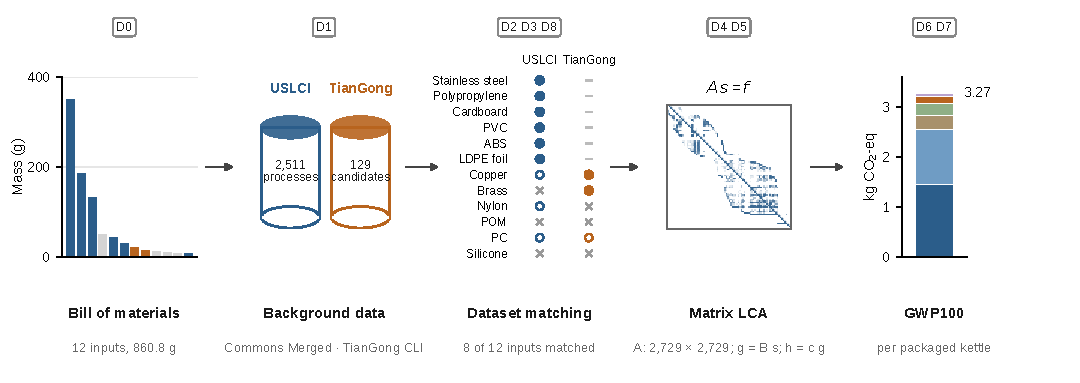
\includegraphics[width=\linewidth]{../figures/report/fig1_method_overview.pdf}
\caption{계산 절차. 매칭 표의 채운 원은 사용한 데이터셋, 빈 원은 검토 후 제외한 후보, $\times$는 데이터 없음, 짧은 선은 검색하지 않음을 뜻한다. 행렬 $A$는 0이 아닌 원소의 위치를 reverse Cuthill--McKee 순서로 표시했다. D0--D8은 표~1의 판단 지점이다.}
\end{figure}

\subsection{특성화와 판단 사항}
특성화는 Commons Merged에 포함된 FEDEFL 기준 IPCC 방법의 AR6-100 범주(CO$_2$ 1, CH$_4$ 29.8, N$_2$O 273)를 사용했다. 생물기원 CO$_2$는 흡수와 배출을 모두 0으로 두었다. 폐기 단계가 경계 밖이므로 흡수 크레딧만 남는 것을 피하기 위해서다. TianGong 흐름은 이름으로 같은 계수에 대응시켰다. 결과에 영향을 주는 판단은 표~1과 같다.

\begin{table}[H]
\small
\caption{판단 사항과 결과 영향}
\begin{tabularx}{\linewidth}{@{}l>{\raggedright\arraybackslash}p{24mm}LL>{\raggedright\arraybackslash}p{36mm}@{}}
\toprule
번호 & 항목 & 채택 & 대안 & 결과 영향 \\
\midrule
D0 & 재료 손실 & PP만 데이터셋 손실률(3.4\%) 적용 & 재료별 손실률 & 미평가(과소 추정 방향) \\
D1 & USLCI 패키지 & Commons Merged & USLCI 단독 & 단독 시 전력 연결 끊김 \\
D2 & 데이터 없는 소재 & 미계산으로 보고 & 금액 기반 또는 문헌 계수 & 미평가 \\
D3 & 부품 가공 & PP 사출 데이터로 다른 수지 가공 대체 & 재질별 가공 데이터 & 미평가 \\
D4 & 다중 산출 공정 & 제품별 열 분리 & 단일 열 연결 & 단일 열 시 PP 수지 117 kg CO$_2$-eq/kg(오류) \\
D5 & 특성화 방법 & AR6-100, 생물기원 CO$_2$ = 0 & AR5-100, Net Biogenic & $+$0.02\%, $+$0.05\% \\
D6 & 스테인리스 스크랩 & value of scrap 부담 유지 & cut-off(무부담) & $-$19.5\% \\
D7 & 골판지 공장 CO$_2$ & 원자료대로 화석 CO$_2$ & 생물기원으로 해석 & $-$7.4\% \\
D8 & 구리·황동 & TianGong 중국 데이터 & USLCI 금액 기반 bridge & 미평가 \\
\bottomrule
\end{tabularx}
\end{table}

\section{결과}
\subsection{총량과 구성}
계산된 항목의 GWP100은 3.27 kg CO$_2$-eq/대이다. 스테인리스강은 질량의 22\%이지만 배출의 44\%를 차지한다. kg당 배출 강도가 7.8 kg CO$_2$-eq로 다른 재료(2.1--4.3 kg CO$_2$-eq/kg)보다 높기 때문이다(그림~2). 폴리프로필렌은 질량 비중이 가장 크며(41\%), 기여의 3분의 1은 사출 가공에서 나온다.

\begin{figure}[H]
\centering
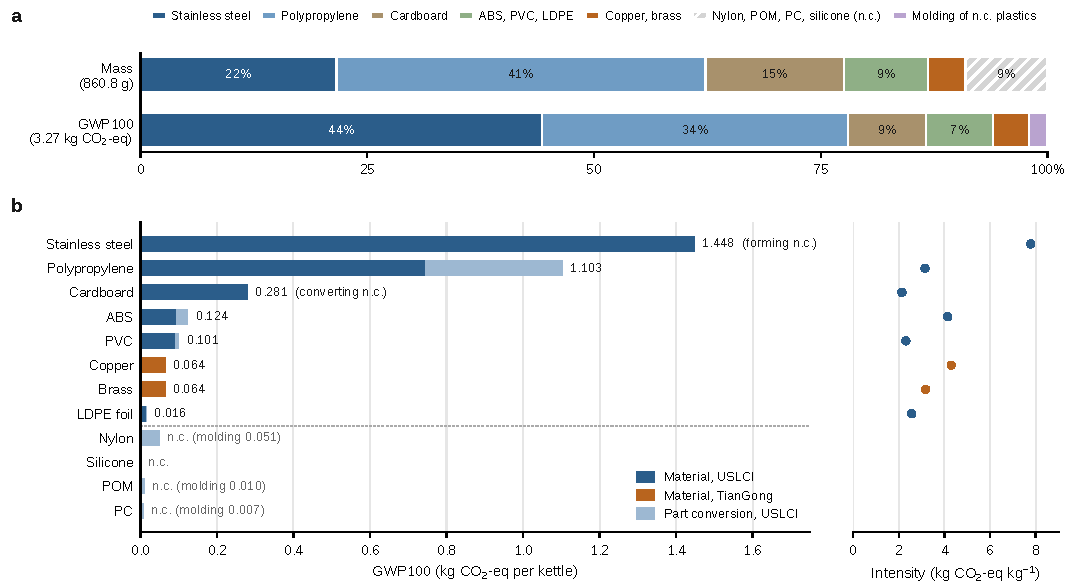
\includegraphics[width=\linewidth]{../figures/report/fig2_results.pdf}
\caption{\textbf{a}, 질량과 GWP100의 구성 비교. 빗금은 미계산 소재의 질량이다. \textbf{b}, 항목별 GWP100과 kg당 배출 강도. 점선 아래 소재는 미계산이며 0이 아니다(n.c.).}
\end{figure}

\begin{table}[H]
\small
\caption{항목별 GWP100 (kg CO$_2$-eq/대)}
\begin{tabularx}{\linewidth}{@{}Lrrrrrl@{}}
\toprule
항목 & 질량(g) & 소재 & 가공 & 합계 & 비율(\%) & 데이터 \\
\midrule
스테인리스강 & 186.00 & 1.448 & -- & 1.448 & 44.3 & USLCI \\
폴리프로필렌(PP) & 350.25 & 0.745 & 0.358 & 1.103 & 33.7 & USLCI \\
골판지(포장) & 131.50 & 0.281 & -- & 0.281 & 8.6 & USLCI \\
ABS & 30.00 & 0.094 & 0.031 & 0.124 & 3.8 & USLCI \\
PVC & 43.50 & 0.092 & 0.009 & 0.101 & 3.1 & USLCI \\
구리 & 15.00 & 0.064 & -- & 0.064 & 2.0 & TianGong \\
황동 & 20.25 & 0.064 & -- & 0.064 & 2.0 & TianGong \\
LDPE 필름(포장) & 6.30 & 0.015 & 0.001 & 0.016 & 0.5 & USLCI \\
나일론(등급 미지정) & 49.50 & 미계산 & 0.051 & -- & -- & 없음 \\
실리콘 & 12.00 & 미계산 & 미계산 & -- & -- & 없음 \\
POM & 9.75 & 미계산 & 0.010 & -- & -- & 없음 \\
PC & 6.75 & 미계산 & 0.007 & -- & -- & 없음 \\
\midrule
\textbf{합계} (GWP는 계산된 항목만) & 860.80 & & & \textbf{3.2691} & 100.0 & \\
\bottomrule
\end{tabularx}
\end{table}

\subsection{공급망 배출원}
공정별 직접 배출로 보면 스테인리스 코일 생산과 스크랩 투입 부담, 골판지 원지 공장, 프로필렌 생산, 에틸렌 크래커의 천연가스 보일러가 상위를 차지한다(그림~3). TianGong 항목(구리, 황동)은 집계 인벤토리이므로 공정별로 분해하지 않았다.

\begin{figure}[H]
\centering
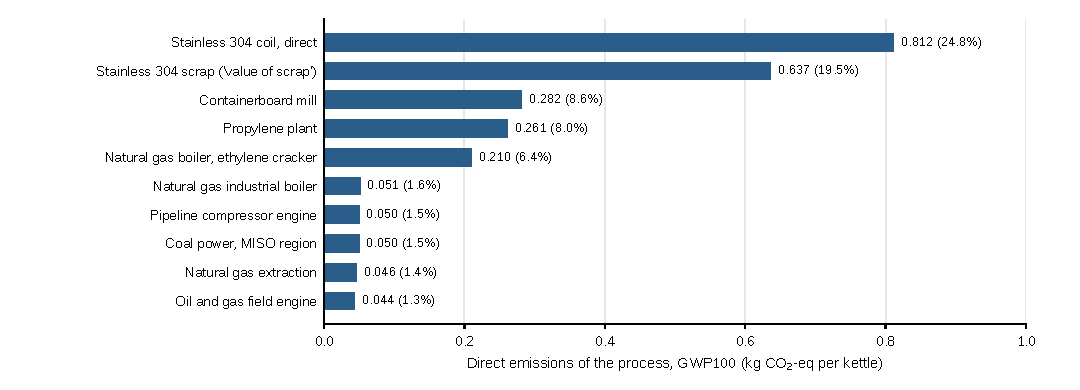
\includegraphics[width=\linewidth]{../figures/report/fig3_hotspots.pdf}
\caption{USLCI 공급망의 공정별 직접 배출 상위 10개. 괄호는 계산된 항목 합계에 대한 비율이다.}
\end{figure}

\subsection{판단별 민감도와 온실가스 구성}
판단 하나를 바꾸면 결과가 최대 $-$19.5\% 달라진다(스테인리스 스크랩 cut-off). 두 판단(D6, D7)을 함께 바꾸면 $-$26.9\%이다. 특성화 방법에 따른 차이는 0.1\% 미만이다. 배출의 90.4\%는 화석 CO$_2$이고, CH$_4$ 8.2\%, N$_2$O 1.4\%이다(그림~4).

\begin{figure}[H]
\centering
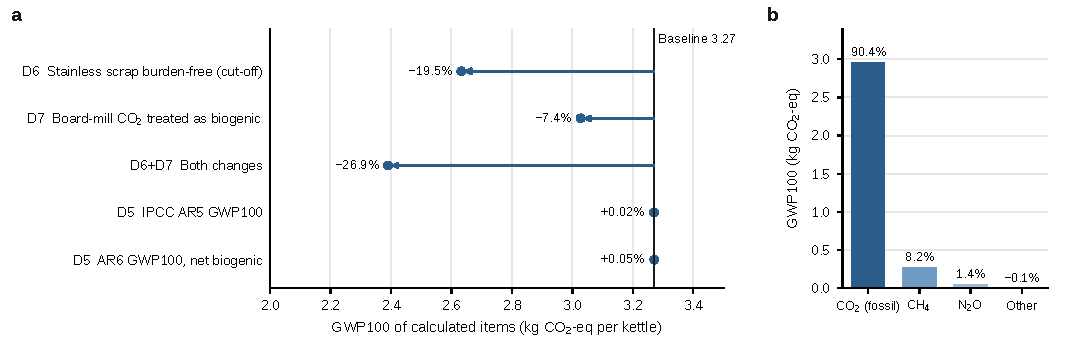
\includegraphics[width=\linewidth]{../figures/report/fig4_decisions_gases.pdf}
\caption{\textbf{a}, 판단 하나를 바꿨을 때의 결과. 세로선은 기준 결과이다. \textbf{b}, 온실가스 종류별 GWP100.}
\end{figure}

\subsection{점검}
\begin{itemize}[leftmargin=12pt,itemsep=1pt]
\item BOM 질량 수지: 723.00 g + 137.80 g = 860.80 g, 일치.
\item 항목별 결과의 합과 전체 행렬 해: 차이 $10^{-9}$ 미만, 일치.
\item 다중 산출 공정을 단일 열로 연결한 초기 구현에서 PP 수지가 117 kg CO$_2$-eq/kg로 과대 산정되는 오류를 발견해 수정했다(수정 후 2.06).
\item USLCI 아연 데이터셋은 0.003 kg CO$_2$-eq/kg로 비정상이어서 사용하지 않았다.
\item 공급자가 없는 투입은 cut-off하고 목록으로 보고했다(results/pass1/unresolved\_links.csv).
\end{itemize}

\section{한계와 미결정 사항}
\begin{enumerate}[leftmargin=14pt,itemsep=1pt]
\item 나일론, POM, PC, 실리콘은 두 DB에 데이터셋이 없다. 금액 기반 USEEIO proxy, 문헌 계수, 누락 보고 중 선택이 필요하다.
\item 나일론 등급(PA6, PA66)과 제조 지역이 정해지지 않았다. USLCI 항목은 미국, TianGong 항목은 중국 데이터이다.
\item 재생 원료 처리가 일관되지 않다. 스테인리스 스크랩은 부담을 유지했고(D6) 황동의 재생 구리는 무부담으로 두었다.
\item 황동 값({3.18} kg CO$_2$-eq/kg)에는 아연 0.35 kg/kg의 배출이 빠져 있다. 구리({4.30} kg CO$_2$-eq/kg)는 투입 석탄의 상류 배출이 연결되지 않아 과소 추정일 수 있다. 중국 전력은 {0.568} kg CO$_2$/kWh(CO$_2$만 기록)이다.
\item 금속 성형, 골판지 상자 가공, 조립 전력, 원료 입고 운송, 재료 손실률(PP 제외)이 반영되지 않았다.
\end{enumerate}

\end{document}
